\documentclass{standalone}
\usepackage{tikz}
\usetikzlibrary{positioning}

\begin{document}
	
	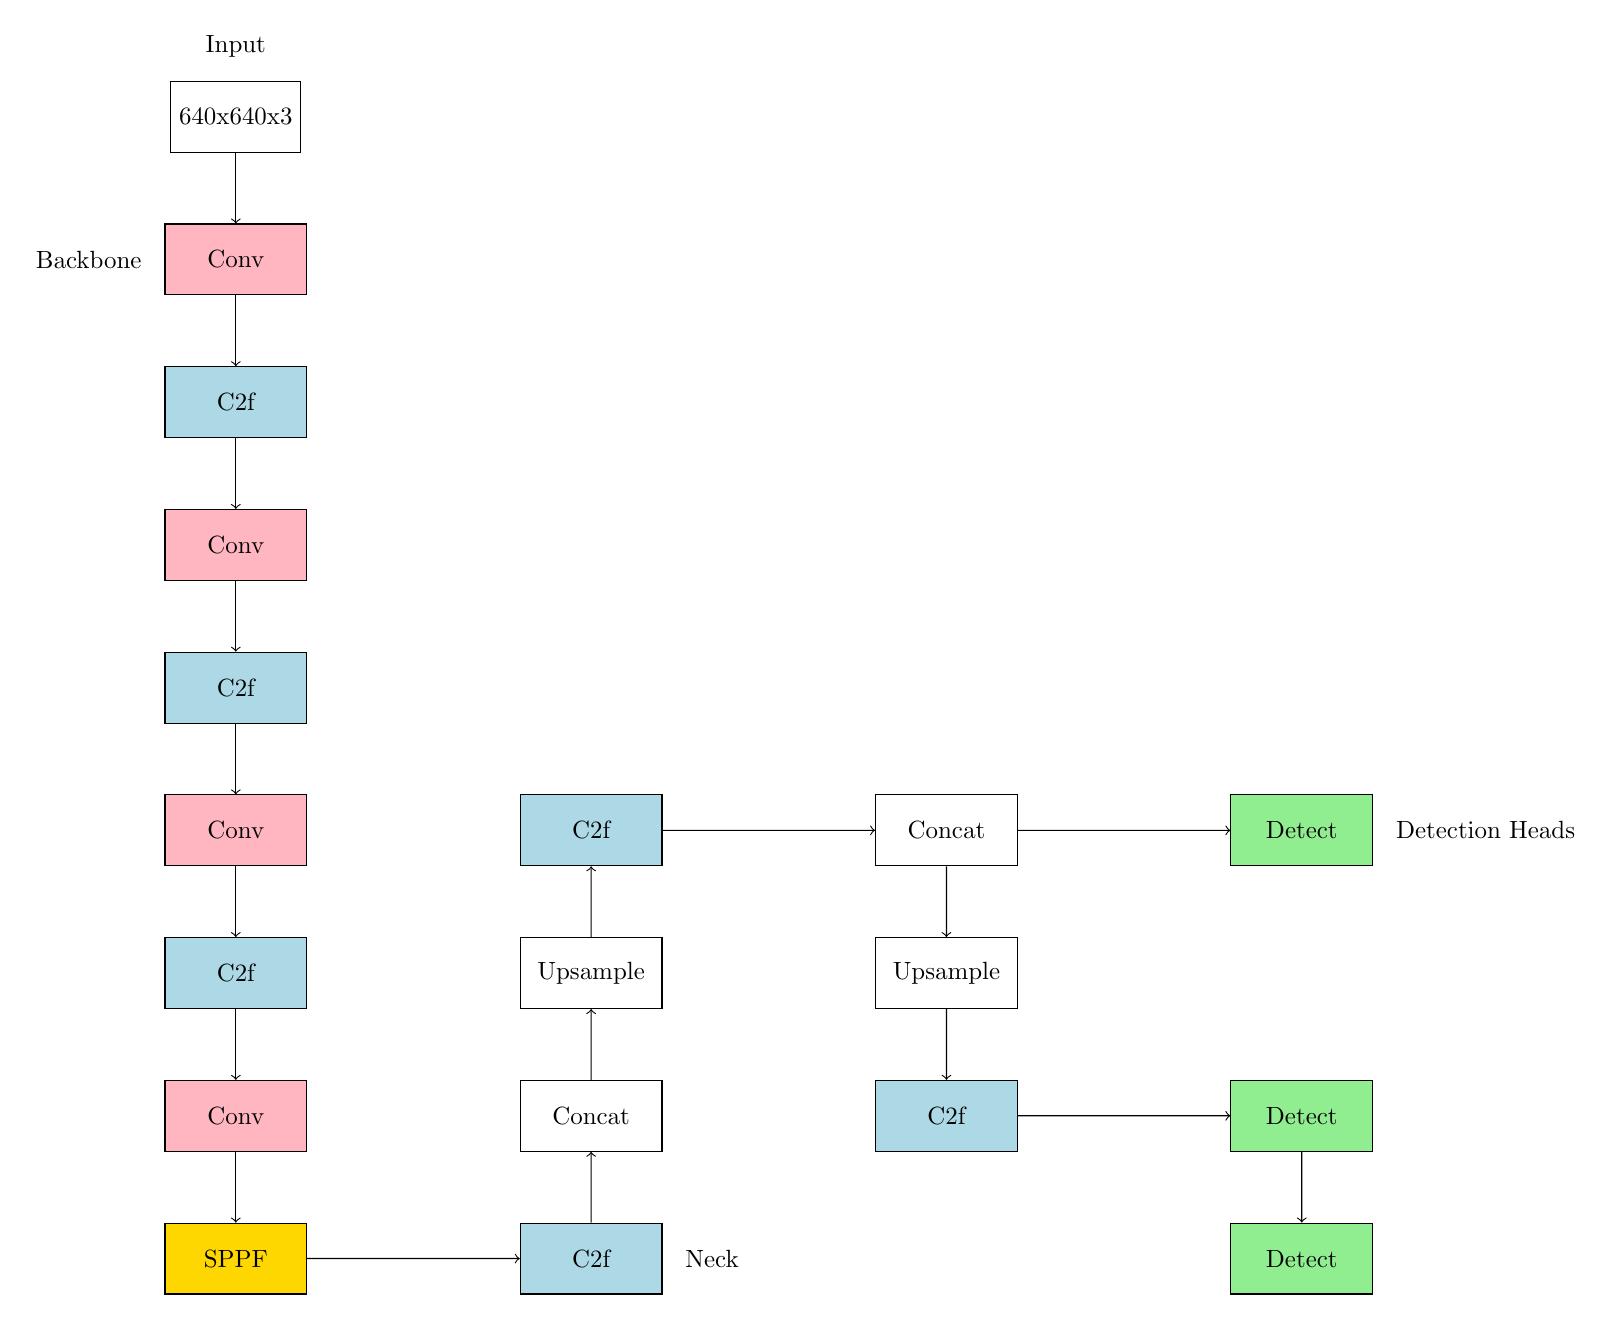
\begin{tikzpicture}[scale=0.9, transform shape]
		
		% Colors
		\definecolor{convcolor}{RGB}{255,182,193} % LightPink
		\definecolor{c2fcolor}{RGB}{173,216,230} % LightBlue
		\definecolor{sppfcolor}{RGB}{255,215,0} % Gold
		\definecolor{detectcolor}{RGB}{144,238,144} % LightGreen
		
		% Input
		\node (input) [draw, rectangle, minimum width=1.5cm, minimum height=1cm] {640x640x3};
		
		% Backbone
		\node (conv1) [draw, rectangle, fill=convcolor, minimum width=2cm, minimum height=1cm, below=1cm of input] {Conv};
		\node (c2f1) [draw, rectangle, fill=c2fcolor, minimum width=2cm, minimum height=1cm, below=1cm of conv1] {C2f};
		\node (conv2) [draw, rectangle, fill=convcolor, minimum width=2cm, minimum height=1cm, below=1cm of c2f1] {Conv};
		\node (c2f2) [draw, rectangle, fill=c2fcolor, minimum width=2cm, minimum height=1cm, below=1cm of conv2] {C2f};
		\node (conv3) [draw, rectangle, fill=convcolor, minimum width=2cm, minimum height=1cm, below=1cm of c2f2] {Conv};
		\node (c2f3) [draw, rectangle, fill=c2fcolor, minimum width=2cm, minimum height=1cm, below=1cm of conv3] {C2f};
		\node (conv4) [draw, rectangle, fill=convcolor, minimum width=2cm, minimum height=1cm, below=1cm of c2f3] {Conv};
		\node (sppf) [draw, rectangle, fill=sppfcolor, minimum width=2cm, minimum height=1cm, below=1cm of conv4] {SPPF};
		
		% Neck
		\node (c2f4) [draw, rectangle, fill=c2fcolor, minimum width=2cm, minimum height=1cm, right=3cm of sppf] {C2f};
		\node (concat1) [draw, rectangle, minimum width=2cm, minimum height=1cm, above=1cm of c2f4] {Concat};
		\node (upsample1) [draw, rectangle, minimum width=2cm, minimum height=1cm, above=1cm of concat1] {Upsample};
		\node (c2f5) [draw, rectangle, fill=c2fcolor, minimum width=2cm, minimum height=1cm, above=1cm of upsample1] {C2f};
		\node (concat2) [draw, rectangle, minimum width=2cm, minimum height=1cm, right=3cm of c2f5] {Concat};
		\node (upsample2) [draw, rectangle, minimum width=2cm, minimum height=1cm, below=1cm of concat2] {Upsample};
		\node (c2f6) [draw, rectangle, fill=c2fcolor, minimum width=2cm, minimum height=1cm, below=1cm of upsample2] {C2f};
		
		% Detection Heads
		\node (detect1) [draw, rectangle, fill=detectcolor, minimum width=2cm, minimum height=1cm, right=3cm of concat2] {Detect};
		\node (detect2) [draw, rectangle, fill=detectcolor, minimum width=2cm, minimum height=1cm, right=3cm of c2f6] {Detect};
		\node (detect3) [draw, rectangle, fill=detectcolor, minimum width=2cm, minimum height=1cm, below=1cm of detect2] {Detect};
		
		% Connections
		\draw[->] (input) -- (conv1);
		\draw[->] (conv1) -- (c2f1);
		\draw[->] (c2f1) -- (conv2);
		\draw[->] (conv2) -- (c2f2);
		\draw[->] (c2f2) -- (conv3);
		\draw[->] (conv3) -- (c2f3);
		\draw[->] (c2f3) -- (conv4);
		\draw[->] (conv4) -- (sppf);
		
		\draw[->] (sppf) -- (c2f4);
		\draw[->] (c2f4) -- (concat1);
		\draw[->] (concat1) -- (upsample1);
		\draw[->] (upsample1) -- (c2f5);
		\draw[->] (c2f5) -- (concat2);
		\draw[->] (concat2) -- (upsample2);
		\draw[->] (upsample2) -- (c2f6);
		
		\draw[->] (concat2) -- (detect1);
		\draw[->] (c2f6) -- (detect2);
		\draw[->] (detect2) -- (detect3);
		
		% Labels
		\node[above=0.2cm] at (input.north) {Input};
		\node[left=0.2cm] at (conv1.west) {Backbone};
		\node[right=0.2cm] at (c2f4.east) {Neck};
		\node[right=0.2cm] at (detect1.east) {Detection Heads};
		
	\end{tikzpicture}
\end{document}
